\documentclass{article} % For LaTeX2e
\usepackage{iclr2024_conference,times}

\usepackage[utf8]{inputenc} % allow utf-8 input
\usepackage[T1]{fontenc}    % use 8-bit T1 fonts
\usepackage{hyperref}       % hyperlinks
\usepackage{url}            % simple URL typesetting
\usepackage{booktabs}       % professional-quality tables
\usepackage{amsfonts}       % blackboard math symbols
\usepackage{nicefrac}       % compact symbols for 1/2, etc.
\usepackage{microtype}      % microtypography
\usepackage{titletoc}

\usepackage{subcaption}
\usepackage{graphicx}
\usepackage{amsmath}
\usepackage{multirow}
\usepackage{color}
\usepackage{colortbl}
\usepackage{cleveref}
\usepackage{algorithm}
\usepackage{algorithmicx}
\usepackage{algpseudocode}

\DeclareMathOperator*{\argmin}{arg\,min}
\DeclareMathOperator*{\argmax}{arg\,max}

\graphicspath{{../}} % To reference your generated figures, see below.
\begin{filecontents}{references.bib}

@book{goodfellow2016deep,
  title={Deep learning},
  author={Goodfellow, Ian and Bengio, Yoshua and Courville, Aaron and Bengio, Yoshua},
  volume={1},
  year={2016},
  publisher={MIT Press}
}

@article{vaswani2017attention,
  title={Attention is all you need},
  author={Vaswani, Ashish and Shazeer, Noam and Parmar, Niki and Uszkoreit, Jakob and Jones, Llion and Gomez, Aidan N and Kaiser, {\L}ukasz and Polosukhin, Illia},
  journal={Advances in neural information processing systems},
  volume={30},
  year={2017}
}

@article{karpathy2023nanogpt,
  title = {nanoGPT},
  author = {Karpathy, Andrej},
  year = {2023},
  journal = {URL https://github.com/karpathy/nanoGPT/tree/master},
  note = {GitHub repository}
}

@article{kingma2014adam,
  title={Adam: A method for stochastic optimization},
  author={Kingma, Diederik P and Ba, Jimmy},
  journal={arXiv preprint arXiv:1412.6980},
  year={2014}
}

@article{ba2016layer,
  title={Layer normalization},
  author={Ba, Jimmy Lei and Kiros, Jamie Ryan and Hinton, Geoffrey E},
  journal={arXiv preprint arXiv:1607.06450},
  year={2016}
}

@article{loshchilov2017adamw,
  title={Decoupled weight decay regularization},
  author={Loshchilov, Ilya and Hutter, Frank},
  journal={arXiv preprint arXiv:1711.05101},
  year={2017}
}

@article{radford2019language,
  title={Language Models are Unsupervised Multitask Learners},
  author={Radford, Alec and Wu, Jeff and Child, Rewon and Luan, David and Amodei, Dario and Sutskever, Ilya},
  year={2019}
}

@article{bahdanau2014neural,
  title={Neural machine translation by jointly learning to align and translate},
  author={Bahdanau, Dzmitry and Cho, Kyunghyun and Bengio, Yoshua},
  journal={arXiv preprint arXiv:1409.0473},
  year={2014}
}

@article{paszke2019pytorch,
  title={Pytorch: An imperative style, high-performance deep learning library},
  author={Paszke, Adam and Gross, Sam and Massa, Francisco and Lerer, Adam and Bradbury, James and Chanan, Gregory and Killeen, Trevor and Lin, Zeming and Gimelshein, Natalia and Antiga, Luca and others},
  journal={Advances in neural information processing systems},
  volume={32},
  year={2019}
}

@misc{gpt4,
  title={GPT-4 Technical Report}, 
  author={OpenAI},
  year={2024},
  eprint={2303.08774},
  archivePrefix={arXiv},
  primaryClass={cs.CL},
  url={https://arxiv.org/abs/2303.08774}, 
}

@misc{bussmannBatchTopKSparseAutoencoders2024,
  title = {{{BatchTopK Sparse Autoencoders}}},
  author = {Bussmann, Bart and Leask, Patrick and Nanda, Neel},
  year = {2024},
  month = dec,
  number = {arXiv:2412.06410},
  eprint = {2412.06410},
  primaryclass = {cs},
  publisher = {arXiv},
  doi = {10.48550/arXiv.2412.06410},
  urldate = {2025-01-06},
  abstract = {Sparse autoencoders (SAEs) have emerged as a powerful tool for interpreting language model activations by decomposing them into sparse, interpretable features. A popular approach is the TopK SAE, that uses a fixed number of the most active latents per sample to reconstruct the model activations. We introduce BatchTopK SAEs, a training method that improves upon TopK SAEs by relaxing the topk constraint to the batch-level, allowing for a variable number of latents to be active per sample. As a result, BatchTopK adaptively allocates more or fewer latents depending on the sample, improving reconstruction without sacrificing average sparsity. We show that BatchTopK SAEs consistently outperform TopK SAEs in reconstructing activations from GPT-2 Small and Gemma 2 2B, and achieve comparable performance to state-of-the-art JumpReLU SAEs. However, an advantage of BatchTopK is that the average number of latents can be directly specified, rather than approximately tuned through a costly hyperparameter sweep. We provide code for training and evaluating BatchTopK SAEs at https://github. com/bartbussmann/BatchTopK.},
  archiveprefix = {arXiv},
  langid = {english},
  keywords = {Computer Science - Artificial Intelligence,Computer Science - Machine Learning,Statistics - Machine Learning},
  file = {C:\Users\yanch\Zotero\storage\EJ5UBSNH\Bussmann et al. - 2024 - BatchTopK Sparse Autoencoders.pdf}
}

@misc{chaninAbsorptionStudyingFeature2024,
  title = {A Is for {{Absorption}}: {{Studying Feature Splitting}} and {{Absorption}} in {{Sparse Autoencoders}}},
  shorttitle = {A Is for {{Absorption}}},
  author = {Chanin, David and {Wilken-Smith}, James and Dulka, Tom{\'a}{\v s} and Bhatnagar, Hardik and Bloom, Joseph},
  year = {2024},
  month = sep,
  number = {arXiv:2409.14507},
  eprint = {2409.14507},
  primaryclass = {cs},
  publisher = {arXiv},
  doi = {10.48550/arXiv.2409.14507},
  urldate = {2025-01-27},
  abstract = {Sparse Autoencoders (SAEs) have emerged as a promising approach to decompose the activations of Large Language Models (LLMs) into human-interpretable latents. In this paper, we pose two questions. First, to what extent do SAEs extract monosemantic and interpretable latents? Second, to what extent does varying the sparsity or the size of the SAE affect monosemanticity / interpretability? By investigating these questions in the context of a simple first-letter identification task where we have complete access to ground truth labels for all tokens in the vocabulary, we are able to provide more detail than prior investigations. Critically, we identify a problematic form of feature-splitting we call feature absorption where seemingly monosemantic latents fail to fire in cases where they clearly should. Our investigation suggests that varying SAE size or sparsity is insufficient to solve this issue, and that there are deeper conceptual issues in need of resolution.},
  archiveprefix = {arXiv},
  keywords = {Computer Science - Artificial Intelligence,Computer Science - Computation and Language},
  file = {C\:\\Users\\yanch\\Zotero\\storage\\QIA3MHNG\\Chanin et al. - 2024 - A is for Absorption Studying Feature Splitting an.pdf;C\:\\Users\\yanch\\Zotero\\storage\\FHXMI5CJ\\2409.html}
}

@inproceedings{de-arteagaBiasBiosCase2019,
  title = {Bias in {{Bios}}: {{A Case Study}} of {{Semantic Representation Bias}} in a {{High-Stakes Setting}}},
  shorttitle = {Bias in {{Bios}}},
  booktitle = {Proceedings of the {{Conference}} on {{Fairness}}, {{Accountability}}, and {{Transparency}}},
  author = {{De-Arteaga}, Maria and Romanov, Alexey and Wallach, Hanna and Chayes, Jennifer and Borgs, Christian and Chouldechova, Alexandra and Geyik, Sahin and Kenthapadi, Krishnaram and Kalai, Adam Tauman},
  year = {2019},
  month = jan,
  eprint = {1901.09451},
  primaryclass = {cs},
  pages = {120--128},
  doi = {10.1145/3287560.3287572},
  urldate = {2025-01-27},
  abstract = {We present a large-scale study of gender bias in occupation classification, a task where the use of machine learning may lead to negative outcomes on peoples' lives. We analyze the potential allocation harms that can result from semantic representation bias. To do so, we study the impact on occupation classification of including explicit gender indicators---such as first names and pronouns---in different semantic representations of online biographies. Additionally, we quantify the bias that remains when these indicators are "scrubbed," and describe proxy behavior that occurs in the absence of explicit gender indicators. As we demonstrate, differences in true positive rates between genders are correlated with existing gender imbalances in occupations, which may compound these imbalances.},
  archiveprefix = {arXiv},
  keywords = {Computer Science - Information Retrieval,Computer Science - Machine Learning,Statistics - Machine Learning},
  note = {Comment: Accepted at ACM Conference on Fairness, Accountability, and Transparency (ACM FAT*), 2019},
  file = {C\:\\Users\\yanch\\Zotero\\storage\\SVU9T3AL\\De-Arteaga et al. - 2019 - Bias in Bios A Case Study of Semantic Representat.pdf;C\:\\Users\\yanch\\Zotero\\storage\\MELZABAJ\\1901.html}
}

@misc{farrellApplyingSparseAutoencoders2024,
  title = {Applying Sparse Autoencoders to Unlearn Knowledge in Language Models},
  author = {Farrell, Eoin and Lau, Yeu-Tong and Conmy, Arthur},
  year = {2024},
  month = nov,
  number = {arXiv:2410.19278},
  eprint = {2410.19278},
  primaryclass = {cs},
  publisher = {arXiv},
  doi = {10.48550/arXiv.2410.19278},
  urldate = {2025-01-27},
  abstract = {We investigate whether sparse autoencoders (SAEs) can be used to remove knowledge from language models. We use the biology subset of the Weapons of Mass Destruction Proxy dataset and test on the gemma-2b-it and gemma-2-2b-it language models. We demonstrate that individual interpretable biology-related SAE features can be used to unlearn a subset of WMDP-Bio questions with minimal side-effects in domains other than biology. Our results suggest that negative scaling of feature activations is necessary and that zero ablating features is ineffective. We find that intervening using multiple SAE features simultaneously can unlearn multiple different topics, but with similar or larger unwanted side-effects than the existing Representation Misdirection for Unlearning technique. Current SAE quality or intervention techniques would need to improve to make SAE-based unlearning comparable to the existing fine-tuning based techniques.},
  archiveprefix = {arXiv},
  keywords = {Computer Science - Artificial Intelligence,Computer Science - Machine Learning},
  file = {C\:\\Users\\yanch\\Zotero\\storage\\534ACMZM\\Farrell et al. - 2024 - Applying sparse autoencoders to unlearn knowledge .pdf;C\:\\Users\\yanch\\Zotero\\storage\\2Z3V2URS\\2410.html}
}

@article{gaoScalingEvaluatingSparse,
  title = {Scaling and Evaluating Sparse Autoencoders},
  author = {Gao, Leo and Goh, Gabriel and Sutskever, Ilya},
  langid = {english},
  file = {C:\Users\yanch\Zotero\storage\W35ULTM4\Gao et al. - Scaling and evaluating sparse autoencoders.pdf}
}

@misc{ghilardiEfficientTrainingSparse2024a,
  title = {Efficient {{Training}} of {{Sparse Autoencoders}} for {{Large Language Models}} via {{Layer Groups}}},
  author = {Ghilardi, Davide and Belotti, Federico and Molinari, Marco},
  year = {2024},
  month = oct,
  number = {arXiv:2410.21508},
  eprint = {2410.21508},
  primaryclass = {cs},
  publisher = {arXiv},
  doi = {10.48550/arXiv.2410.21508},
  urldate = {2025-01-06},
  abstract = {Sparse Autoencoders (SAEs) have recently been employed as an unsupervised approach for understanding the inner workings of Large Language Models (LLMs). They reconstruct the model's activations with a sparse linear combination of interpretable features. However, training SAEs is computationally intensive, especially as models grow in size and complexity. To address this challenge, we propose a novel training strategy that reduces the number of trained SAEs from one per layer to one for a given group of contiguous layers. Our experimental results on Pythia 160M highlight a speedup of up to 6x without compromising the reconstruction quality and performance on downstream tasks. Therefore, layer clustering presents an efficient approach to train SAEs in modern LLMs.},
  archiveprefix = {arXiv},
  langid = {english},
  keywords = {Computer Science - Artificial Intelligence,Computer Science - Computation and Language},
  file = {C:\Users\yanch\Zotero\storage\HCBUHHAA\Ghilardi et al. - 2024 - Efficient Training of Sparse Autoencoders for Larg.pdf}
}

@misc{gurneeFindingNeuronsHaystack2023,
  title = {Finding {{Neurons}} in a {{Haystack}}: {{Case Studies}} with {{Sparse Probing}}},
  shorttitle = {Finding {{Neurons}} in a {{Haystack}}},
  author = {Gurnee, Wes and Nanda, Neel and Pauly, Matthew and Harvey, Katherine and Troitskii, Dmitrii and Bertsimas, Dimitris},
  year = {2023},
  month = jun,
  number = {arXiv:2305.01610},
  eprint = {2305.01610},
  primaryclass = {cs},
  publisher = {arXiv},
  doi = {10.48550/arXiv.2305.01610},
  urldate = {2025-01-27},
  abstract = {Despite rapid adoption and deployment of large language models (LLMs), the internal computations of these models remain opaque and poorly understood. In this work, we seek to understand how high-level human-interpretable features are represented within the internal neuron activations of LLMs. We train \$k\$-sparse linear classifiers (probes) on these internal activations to predict the presence of features in the input; by varying the value of \$k\$ we study the sparsity of learned representations and how this varies with model scale. With \$k=1\$, we localize individual neurons which are highly relevant for a particular feature, and perform a number of case studies to illustrate general properties of LLMs. In particular, we show that early layers make use of sparse combinations of neurons to represent many features in superposition, that middle layers have seemingly dedicated neurons to represent higher-level contextual features, and that increasing scale causes representational sparsity to increase on average, but there are multiple types of scaling dynamics. In all, we probe for over 100 unique features comprising 10 different categories in 7 different models spanning 70 million to 6.9 billion parameters.},
  archiveprefix = {arXiv},
  keywords = {Computer Science - Artificial Intelligence,Computer Science - Machine Learning},
  file = {C\:\\Users\\yanch\\Zotero\\storage\\9B43DKLD\\Gurnee et al. - 2023 - Finding Neurons in a Haystack Case Studies with S.pdf;C\:\\Users\\yanch\\Zotero\\storage\\VTA4Y7RU\\2305.html}
}

@misc{InterpretabilityCompressionReconsidering,
  title = {Interpretability as {{Compression}}: {{Reconsidering SAE Explanations}} of {{Neural Activations}} with {{MDL-SAEs}}},
  urldate = {2025-01-15},
  howpublished = {https://arxiv.org/html/2410.11179v1},
  file = {C:\Users\yanch\Zotero\storage\S3LK2LEB\2410.html}
}

@misc{karvonenEvaluatingSparseAutoencoders2024,
  title = {Evaluating {{Sparse Autoencoders}} on {{Targeted Concept Erasure Tasks}}},
  author = {Karvonen, Adam and Rager, Can and Marks, Samuel and Nanda, Neel},
  year = {2024},
  month = nov,
  number = {arXiv:2411.18895},
  eprint = {2411.18895},
  primaryclass = {cs},
  publisher = {arXiv},
  doi = {10.48550/arXiv.2411.18895},
  urldate = {2025-01-27},
  abstract = {Sparse Autoencoders (SAEs) are an interpretability technique aimed at decomposing neural network activations into interpretable units. However, a major bottleneck for SAE development has been the lack of high-quality performance metrics, with prior work largely relying on unsupervised proxies. In this work, we introduce a family of evaluations based on SHIFT, a downstream task from Marks et al. (Sparse Feature Circuits, 2024) in which spurious cues are removed from a classifier by ablating SAE features judged to be task-irrelevant by a human annotator. We adapt SHIFT into an automated metric of SAE quality; this involves replacing the human annotator with an LLM. Additionally, we introduce the Targeted Probe Perturbation (TPP) metric that quantifies an SAE's ability to disentangle similar concepts, effectively scaling SHIFT to a wider range of datasets. We apply both SHIFT and TPP to multiple open-source models, demonstrating that these metrics effectively differentiate between various SAE training hyperparameters and architectures.},
  archiveprefix = {arXiv},
  keywords = {Computer Science - Computation and Language,Computer Science - Machine Learning},
  file = {C\:\\Users\\yanch\\Zotero\\storage\\HRKJ9X7I\\Karvonen et al. - 2024 - Evaluating Sparse Autoencoders on Targeted Concept.pdf;C\:\\Users\\yanch\\Zotero\\storage\\7P5P4TUP\\2411.html}
}

@misc{liWMDPBenchmarkMeasuring2024,
  title = {The {{WMDP Benchmark}}: {{Measuring}} and {{Reducing Malicious Use With Unlearning}}},
  shorttitle = {The {{WMDP Benchmark}}},
  author = {Li, Nathaniel and Pan, Alexander and Gopal, Anjali and Yue, Summer and Berrios, Daniel and Gatti, Alice and Li, Justin D. and Dombrowski, Ann-Kathrin and Goel, Shashwat and Phan, Long and Mukobi, Gabriel and {Helm-Burger}, Nathan and Lababidi, Rassin and Justen, Lennart and Liu, Andrew B. and Chen, Michael and Barrass, Isabelle and Zhang, Oliver and Zhu, Xiaoyuan and Tamirisa, Rishub and Bharathi, Bhrugu and Khoja, Adam and Zhao, Zhenqi and {Herbert-Voss}, Ariel and Breuer, Cort B. and Marks, Samuel and Patel, Oam and Zou, Andy and Mazeika, Mantas and Wang, Zifan and Oswal, Palash and Lin, Weiran and Hunt, Adam A. and {Tienken-Harder}, Justin and Shih, Kevin Y. and Talley, Kemper and Guan, John and Kaplan, Russell and Steneker, Ian and Campbell, David and Jokubaitis, Brad and Levinson, Alex and Wang, Jean and Qian, William and Karmakar, Kallol Krishna and Basart, Steven and Fitz, Stephen and Levine, Mindy and Kumaraguru, Ponnurangam and Tupakula, Uday and Varadharajan, Vijay and Wang, Ruoyu and Shoshitaishvili, Yan and Ba, Jimmy and Esvelt, Kevin M. and Wang, Alexandr and Hendrycks, Dan},
  year = {2024},
  month = may,
  number = {arXiv:2403.03218},
  eprint = {2403.03218},
  primaryclass = {cs},
  publisher = {arXiv},
  doi = {10.48550/arXiv.2403.03218},
  urldate = {2025-01-27},
  abstract = {The White House Executive Order on Artificial Intelligence highlights the risks of large language models (LLMs) empowering malicious actors in developing biological, cyber, and chemical weapons. To measure these risks of malicious use, government institutions and major AI labs are developing evaluations for hazardous capabilities in LLMs. However, current evaluations are private, preventing further research into mitigating risk. Furthermore, they focus on only a few, highly specific pathways for malicious use. To fill these gaps, we publicly release the Weapons of Mass Destruction Proxy (WMDP) benchmark, a dataset of 3,668 multiple-choice questions that serve as a proxy measurement of hazardous knowledge in biosecurity, cybersecurity, and chemical security. WMDP was developed by a consortium of academics and technical consultants, and was stringently filtered to eliminate sensitive information prior to public release. WMDP serves two roles: first, as an evaluation for hazardous knowledge in LLMs, and second, as a benchmark for unlearning methods to remove such hazardous knowledge. To guide progress on unlearning, we develop RMU, a state-of-the-art unlearning method based on controlling model representations. RMU reduces model performance on WMDP while maintaining general capabilities in areas such as biology and computer science, suggesting that unlearning may be a concrete path towards reducing malicious use from LLMs. We release our benchmark and code publicly at https://wmdp.ai},
  archiveprefix = {arXiv},
  keywords = {Computer Science - Artificial Intelligence,Computer Science - Computation and Language,Computer Science - Computers and Society,Computer Science - Machine Learning},
  note = {Comment: See the project page at https://wmdp.ai},
  file = {C\:\\Users\\yanch\\Zotero\\storage\\IH8WJB8J\\Li et al. - 2024 - The WMDP Benchmark Measuring and Reducing Malicio.pdf;C\:\\Users\\yanch\\Zotero\\storage\\PI5CUBZH\\2403.html}
}

@misc{marksSparseFeatureCircuits2024,
  title = {Sparse {{Feature Circuits}}: {{Discovering}} and {{Editing Interpretable Causal Graphs}} in {{Language Models}}},
  shorttitle = {Sparse {{Feature Circuits}}},
  author = {Marks, Samuel and Rager, Can and Michaud, Eric J. and Belinkov, Yonatan and Bau, David and Mueller, Aaron},
  year = {2024},
  month = mar,
  number = {arXiv:2403.19647},
  eprint = {2403.19647},
  primaryclass = {cs},
  publisher = {arXiv},
  doi = {10.48550/arXiv.2403.19647},
  urldate = {2025-01-27},
  abstract = {We introduce methods for discovering and applying sparse feature circuits. These are causally implicated subnetworks of human-interpretable features for explaining language model behaviors. Circuits identified in prior work consist of polysemantic and difficult-to-interpret units like attention heads or neurons, rendering them unsuitable for many downstream applications. In contrast, sparse feature circuits enable detailed understanding of unanticipated mechanisms. Because they are based on fine-grained units, sparse feature circuits are useful for downstream tasks: We introduce SHIFT, where we improve the generalization of a classifier by ablating features that a human judges to be task-irrelevant. Finally, we demonstrate an entirely unsupervised and scalable interpretability pipeline by discovering thousands of sparse feature circuits for automatically discovered model behaviors.},
  archiveprefix = {arXiv},
  keywords = {Computer Science - Artificial Intelligence,Computer Science - Computation and Language,Computer Science - Machine Learning},
  note = {Comment: Code and data at https://github.com/saprmarks/feature-circuits. Demonstration at https://feature-circuits.xyz},
  file = {C\:\\Users\\yanch\\Zotero\\storage\\U9MWC7I4\\Marks et al. - 2024 - Sparse Feature Circuits Discovering and Editing I.pdf;C\:\\Users\\yanch\\Zotero\\storage\\AML7HRZK\\2403.html}
}

@misc{mudideEfficientDictionaryLearning2024a,
  title = {Efficient {{Dictionary Learning}} with {{Switch Sparse Autoencoders}}},
  author = {Mudide, Anish and Engels, Joshua and Michaud, Eric J. and Tegmark, Max and de Witt, Christian Schroeder},
  year = {2024},
  month = oct,
  number = {arXiv:2410.08201},
  eprint = {2410.08201},
  primaryclass = {cs},
  publisher = {arXiv},
  doi = {10.48550/arXiv.2410.08201},
  urldate = {2025-01-06},
  abstract = {Sparse autoencoders (SAEs) are a recent technique for decomposing neural network activations into human-interpretable features. However, in order for SAEs to identify all features represented in frontier models, it will be necessary to scale them up to very high width, posing a computational challenge. In this work, we introduce Switch Sparse Autoencoders, a novel SAE architecture aimed at reducing the compute cost of training SAEs. Inspired by sparse mixture of experts models, Switch SAEs route activation vectors between smaller ``expert'' SAEs, enabling SAEs to efficiently scale to many more features. We present experiments comparing Switch SAEs with other SAE architectures, and find that Switch SAEs deliver a substantial Pareto improvement in the reconstruction vs. sparsity frontier for a given fixed training compute budget. We also study the geometry of features across experts, analyze features duplicated across experts, and verify that Switch SAE features are as interpretable as features found by other SAE architectures.},
  archiveprefix = {arXiv},
  langid = {english},
  keywords = {Computer Science - Machine Learning},
  note = {Comment: Code available at https://github.com/amudide/switch\_sae},
  file = {C:\Users\yanch\Zotero\storage\ZZUFEFUK\Mudide et al. - 2024 - Efficient Dictionary Learning with Switch Sparse A.pdf}
}

@misc{pauloAutomaticallyInterpretingMillions2024,
  title = {Automatically {{Interpreting Millions}} of {{Features}} in {{Large Language Models}}},
  author = {Paulo, Gon{\c c}alo and Mallen, Alex and Juang, Caden and Belrose, Nora},
  year = {2024},
  month = dec,
  number = {arXiv:2410.13928},
  eprint = {2410.13928},
  primaryclass = {cs},
  publisher = {arXiv},
  doi = {10.48550/arXiv.2410.13928},
  urldate = {2025-01-27},
  abstract = {While the activations of neurons in deep neural networks usually do not have a simple human-understandable interpretation, sparse autoencoders (SAEs) can be used to transform these activations into a higher-dimensional latent space which may be more easily interpretable. However, these SAEs can have millions of distinct latent features, making it infeasible for humans to manually interpret each one. In this work, we build an open-source automated pipeline to generate and evaluate natural language explanations for SAE features using LLMs. We test our framework on SAEs of varying sizes, activation functions, and losses, trained on two different open-weight LLMs. We introduce five new techniques to score the quality of explanations that are cheaper to run than the previous state of the art. One of these techniques, intervention scoring, evaluates the interpretability of the effects of intervening on a feature, which we find explains features that are not recalled by existing methods. We propose guidelines for generating better explanations that remain valid for a broader set of activating contexts, and discuss pitfalls with existing scoring techniques. We use our explanations to measure the semantic similarity of independently trained SAEs, and find that SAEs trained on nearby layers of the residual stream are highly similar. Our large-scale analysis confirms that SAE latents are indeed much more interpretable than neurons, even when neurons are sparsified using top-\$k\$ postprocessing. Our code is available at https://github.com/EleutherAI/sae-auto-interp, and our explanations are available at https://huggingface.co/datasets/EleutherAI/auto\_interp\_explanations.},
  archiveprefix = {arXiv},
  keywords = {Computer Science - Computation and Language,Computer Science - Machine Learning},
  file = {C\:\\Users\\yanch\\Zotero\\storage\\7ADXVWT6\\Paulo et al. - 2024 - Automatically Interpreting Millions of Features in.pdf;C\:\\Users\\yanch\\Zotero\\storage\\5HVTWCYX\\2410.html}
}

@misc{rajamanoharanImprovingDictionaryLearning2024,
  title = {Improving {{Dictionary Learning}} with {{Gated Sparse Autoencoders}}},
  author = {Rajamanoharan, Senthooran and Conmy, Arthur and Smith, Lewis and Lieberum, Tom and Varma, Vikrant and Kram{\'a}r, J{\'a}nos and Shah, Rohin and Nanda, Neel},
  year = {2024},
  month = apr,
  number = {arXiv:2404.16014},
  eprint = {2404.16014},
  primaryclass = {cs},
  publisher = {arXiv},
  doi = {10.48550/arXiv.2404.16014},
  urldate = {2025-01-06},
  abstract = {Recent work has found that sparse autoencoders (SAEs) are an effective technique for unsupervised discovery of interpretable features in language models' (LMs) activations, by finding sparse, linear reconstructions of LM activations. We introduce the Gated Sparse Autoencoder (Gated SAE), which achieves a Pareto improvement over training with prevailing methods. In SAEs, the L1 penalty used to encourage sparsity introduces many undesirable biases, such as shrinkage -- systematic underestimation of feature activations. The key insight of Gated SAEs is to separate the functionality of (a) determining which directions to use and (b) estimating the magnitudes of those directions: this enables us to apply the L1 penalty only to the former, limiting the scope of undesirable side effects. Through training SAEs on LMs of up to 7B parameters we find that, in typical hyper-parameter ranges, Gated SAEs solve shrinkage, are similarly interpretable, and require half as many firing features to achieve comparable reconstruction fidelity.},
  archiveprefix = {arXiv},
  langid = {english},
  keywords = {Computer Science - Artificial Intelligence,Computer Science - Machine Learning},
  note = {Comment: 15 main text pages, 22 appendix pages},
  file = {C:\Users\yanch\Zotero\storage\FWEYSUFQ\Rajamanoharan et al. - 2024 - Improving Dictionary Learning with Gated Sparse Au.pdf}
}

@misc{rajamanoharanJumpingAheadImproving2024,
  title = {Jumping {{Ahead}}: {{Improving Reconstruction Fidelity}} with {{JumpReLU Sparse Autoencoders}}},
  shorttitle = {Jumping {{Ahead}}},
  author = {Rajamanoharan, Senthooran and Lieberum, Tom and Sonnerat, Nicolas and Conmy, Arthur and Varma, Vikrant and Kram{\'a}r, J{\'a}nos and Nanda, Neel},
  year = {2024},
  month = aug,
  number = {arXiv:2407.14435},
  eprint = {2407.14435},
  primaryclass = {cs},
  publisher = {arXiv},
  doi = {10.48550/arXiv.2407.14435},
  urldate = {2025-01-06},
  abstract = {Sparse autoencoders (SAEs) are a promising unsupervised approach for identifying causally relevant and interpretable linear features in a language model's (LM) activations. To be useful for downstream tasks, SAEs need to decompose LM activations faithfully; yet to be interpretable the decomposition must be sparse -- two objectives that are in tension. In this paper, we introduce JumpReLU SAEs, which achieve state-of-the-art reconstruction fidelity at a given sparsity level on Gemma 2 9B activations, compared to other recent advances such as Gated and TopK SAEs. We also show that this improvement does not come at the cost of interpretability through manual and automated interpretability studies. JumpReLU SAEs are a simple modification of vanilla (ReLU) SAEs -- where we replace the ReLU with a discontinuous JumpReLU activation function -- and are similarly efficient to train and run. By utilising straight-through-estimators (STEs) in a principled manner, we show how it is possible to train JumpReLU SAEs effectively despite the discontinuous JumpReLU function introduced in the SAE's forward pass. Similarly, we use STEs to directly train L0 to be sparse, instead of training on proxies such as L1, avoiding problems like shrinkage.},
  archiveprefix = {arXiv},
  langid = {english},
  keywords = {Computer Science - Machine Learning},
  note = {Comment: v2: new appendix H comparing kernel functions \& bug-fixes to pseudo-code in Appendix J v3: further bug-fix to pseudo-code in Appendix J},
  file = {C:\Users\yanch\Zotero\storage\Q7MG9Z77\Rajamanoharan et al. - 2024 - Jumping Ahead Improving Reconstruction Fidelity w.pdf}
}

@article{hou2024bridging,
  title={Bridging Language and Items for Retrieval and Recommendation},
  author={Hou, Yupeng and Li, Jiacheng and He, Zhankui and Yan, An and Chen, Xiusi and McAuley, Julian},
  journal={arXiv preprint arXiv:2403.03952},
  year={2024}
}


@Article{Li2024TheWB,
 author = {Nathaniel Li and Alexander Pan and Anjali Gopal and Summer Yue and Daniel Berrios and Alice Gatti and Justin D. Li and Ann-Kathrin Dombrowski and Shashwat Goel and Long Phan and Gabriel Mukobi and Nathan Helm-Burger and Rassin R. Lababidi and Lennart Justen and Andrew B. Liu and Michael Chen and Isabelle Barrass and Oliver Zhang and Xiaoyuan Zhu and Rishub Tamirisa and Bhrugu Bharathi and Adam Khoja and Ariel Herbert-Voss and Cort B. Breuer and Andy Zou and Mantas Mazeika and Zifan Wang and Palash Oswal and Weiran Liu and Adam A. Hunt and Justin Tienken-Harder and Kevin Y. Shih and Kemper Talley and John Guan and Russell Kaplan and Ian Steneker and David Campbell and Brad Jokubaitis and Alex Levinson and Jean Wang and William Qian and K. Karmakar and Steven Basart and Stephen Fitz and Mindy Levine and P. Kumaraguru and U. Tupakula and Vijay Varadharajan and Yan Shoshitaishvili and Jimmy Ba and K. Esvelt and Alexandr Wang and Dan Hendrycks},
 booktitle = {International Conference on Machine Learning},
 journal = {ArXiv},
 title = {The WMDP Benchmark: Measuring and Reducing Malicious Use With Unlearning},
 volume = {abs/2403.03218},
 year = {2024}
}


@Article{Park2024MonetMO,
 author = {Jungwoo Park and Y. Ahn and Kee-Eung Kim and Jaewoo Kang},
 booktitle = {arXiv.org},
 journal = {ArXiv},
 title = {Monet: Mixture of Monosemantic Experts for Transformers},
 volume = {abs/2412.04139},
 year = {2024}
}


@Article{Rajamanoharan2024JumpingAI,
 author = {Senthooran Rajamanoharan and Tom Lieberum and Nicolas Sonnerat and Arthur Conmy and Vikrant Varma and János Kramár and Neel Nanda},
 booktitle = {arXiv.org},
 journal = {ArXiv},
 title = {Jumping Ahead: Improving Reconstruction Fidelity with JumpReLU Sparse Autoencoders},
 volume = {abs/2407.14435},
 year = {2024}
}

\end{filecontents}

\title{HierarchicalSAE: Dynamic Feature Learning for Robust Neural Interpretability}

\author{LLM\\
Department of Computer Science\\
University of LLMs\\
}

\newcommand{\fix}{\marginpar{FIX}}
\newcommand{\new}{\marginpar{NEW}}

\begin{document}

\maketitle

\begin{abstract}
Understanding the internal representations of large language models is crucial for ensuring their reliability and safety, with sparse autoencoders (SAEs) emerging as a promising interpretability approach. However, current SAEs suffer from feature absorption, where learned features inconsistently activate across similar contexts, limiting their reliability for model analysis. We introduce HierarchicalSAE, which combines linear sparsity scheduling with dynamic feature clustering to prevent absorption while maintaining interpretability. Our key innovation is an adaptive sparsity mechanism that automatically adjusts constraints based on reconstruction quality, supported by a sliding window approach for monitoring feature stability. Experiments on Gemma-2-2B demonstrate substantial improvements over standard SAEs: 34\% reduction in feature absorption (from 0.0088 to 0.0058), 7.8 percentage point increase in explained variance (90.2\% vs 82.4\%), and 15.2 percentage point gain in sparse probing accuracy (85.3\% vs 70.1\%). The model maintains 5.4x more active features (1,735 vs 320) while achieving better model preservation (KL divergence 0.058 vs 0.103), enabling more comprehensive and reliable analysis of neural network behavior.
\end{abstract}

\section{Introduction}
\label{sec:intro}

As large language models become increasingly powerful and ubiquitous, understanding their internal representations is crucial for ensuring safety and reliability. Sparse autoencoders (SAEs) have emerged as a promising approach for decomposing neural activations into interpretable features \cite{gaoScalingEvaluatingSparse}, enabling researchers to analyze model behavior at a mechanistic level. However, current interpretability techniques face significant challenges in providing consistent and reliable insights into model behavior, particularly as models scale to billions of parameters.

A fundamental challenge in neural network interpretability is feature absorption \cite{chaninAbsorptionStudyingFeature2024}, where learned features fail to activate consistently across semantically similar contexts. This phenomenon manifests in three key ways:
\begin{itemize}
    \item Inconsistent feature activation despite similar input patterns
    \item Loss of interpretability when scaling to larger feature spaces
    \item Difficulty maintaining both sparsity and reconstruction fidelity
\end{itemize}
Traditional approaches using static sparsity constraints have proven insufficient, with baseline SAEs on Gemma-2-2B showing concerning absorption rates (0.0088) and limited feature utilization (320 active features).

We address these challenges through HierarchicalSAE, a novel architecture that combines dynamic sparsity scheduling with feature clustering. Our key technical innovations are:
\begin{itemize}
    \item Linear sparsity scheduling that automatically adjusts constraints based on reconstruction quality
    \item Proportional window tracking to maintain feature stability and prevent collapse
    \item Adaptive feature clustering that preserves interpretability while reducing redundancy
\end{itemize}

Through extensive experiments on the Gemma-2-2B language model, we demonstrate:
\begin{itemize}
    \item 34\% reduction in feature absorption (score: 0.0058)
    \item 7.8 percentage point increase in explained variance (90.2\%)
    \item 15.2 percentage point gain in sparse probing accuracy (85.3\%)
    \item 5.4x increase in active features (1,735) with improved stability
\end{itemize}

Our main contributions are:
\begin{itemize}
    \item The first SAE architecture specifically designed to prevent feature absorption while maintaining high feature counts
    \item A novel dynamic sparsity mechanism that achieves state-of-the-art reconstruction (90.2\% explained variance) without compromising interpretability
    \item Comprehensive empirical validation across multiple evaluation metrics, including automated interpretation and manual feature inspection
    \item Open-source implementation and evaluation framework for reproducible interpretability research
\end{itemize}

Looking forward, our approach opens new possibilities for analyzing larger models and more complex behaviors. The success of dynamic sparsity scheduling suggests promising directions for addressing other interpretability challenges, such as feature composition and causal analysis. Additionally, our improved feature extraction could enable more targeted interventions for model steering and safety improvements.

\section{Related Work}
\label{sec:related}

Our work builds on recent advances in sparse autoencoder architectures while specifically targeting the feature absorption problem. We organize related work into three categories based on their primary focus: absorption mitigation, architectural innovations, and evaluation methods.

\textbf{Absorption Mitigation:} \cite{chaninAbsorptionStudyingFeature2024} first formalized feature absorption through first-letter identification tasks, showing that traditional approaches like increased model size or adjusted sparsity fail to prevent features from inconsistently activating. While they identified the problem and established baseline metrics (0.0088 absorption rate), they did not propose architectural solutions. Our hierarchical approach directly addresses their findings by dynamically adjusting sparsity constraints based on reconstruction quality.

\textbf{Architectural Innovations:} Several recent works have proposed architectural improvements that complement our approach. BatchTopK SAEs \cite{bussmannBatchTopKSparseAutoencoders2024} relax per-sample sparsity to batch level, achieving 82.4\% explained variance but not addressing absorption. Switch SAEs \cite{mudideEfficientDictionaryLearning2024a} improve computational efficiency through expert routing but maintain static sparsity constraints. JumpReLU \cite{rajamanoharanJumpingAheadImproving2024} and Gated SAEs \cite{rajamanoharanImprovingDictionaryLearning2024} focus on reconstruction fidelity through activation function modifications and magnitude estimation, respectively. While these methods achieve high reconstruction quality, they do not incorporate mechanisms to prevent feature absorption. Our work demonstrates that combining linear sparsity scheduling with feature clustering can maintain their reconstruction benefits while reducing absorption.

\textbf{Evaluation Methods:} Our evaluation builds on two key approaches. \cite{gurneeFindingNeuronsHaystack2023} introduced sparse probing to quantify feature interpretability, which we use to validate our improved feature extraction (85.3\% vs 70.1\% accuracy). \cite{pauloAutomaticallyInterpretingMillions2024} developed automated interpretation techniques that scale to large feature spaces, complementing our ability to maintain more active features (1,735 vs 320) without sacrificing interpretability. These methods provide crucial validation that our absorption prevention mechanisms do not compromise feature quality.

\section{Background}
\label{sec:background}

Sparse autoencoders (SAEs) have emerged as a powerful tool for understanding large language models by decomposing neural activations into interpretable features \cite{gaoScalingEvaluatingSparse}. The core insight is that while individual neurons often encode entangled concepts, linear combinations of activations can isolate semantically meaningful features when properly constrained. This builds on classical work in dictionary learning and sparse coding, adapted to the scale and complexity of modern language models.

Recent work has identified feature absorption as a fundamental challenge in SAE interpretability \cite{chaninAbsorptionStudyingFeature2024}. This phenomenon occurs when semantically unified concepts are inconsistently split across multiple features, or when features fail to activate in relevant contexts despite the presence of their target concept. While architectural innovations like BatchTopK \cite{bussmannBatchTopKSparseAutoencoders2024} and Switch SAEs \cite{mudideEfficientDictionaryLearning2024a} have improved reconstruction quality, they do not directly address the absorption problem.

\subsection{Problem Setting}
Consider a pre-trained language model $\mathcal{M}$ that maps input tokens to hidden states $h \in \mathbb{R}^d$. An SAE consists of an encoder $E: \mathbb{R}^d \to \mathbb{R}^k$ and decoder $D: \mathbb{R}^k \to \mathbb{R}^d$ where $k$ is the dictionary size. The encoder produces sparse activations $z = E(h)$ such that most entries in $z$ are zero, while the decoder attempts to reconstruct the original activations $\hat{h} = D(z)$.

The feature absorption problem manifests in two key ways:
\begin{itemize}
    \item \textbf{Splitting}: A single semantic concept $c$ activates different features $F_c \subseteq [k]$ across different contexts
    \item \textbf{Inconsistency}: A feature $i \in F_c$ fails to activate for some inputs containing concept $c$
\end{itemize}

Formally, we aim to learn $(E,D)$ that optimize:
\begin{align*}
    \mathcal{L}_{\text{recon}} &= \mathbb{E}_h[\|h - D(E(h))\|_2^2] \\
    \mathcal{L}_{\text{sparse}} &= \mathbb{E}_h[\|E(h)\|_1] \\
    \text{s.t.} \quad & \|E(h)\|_0 \ll d \quad \forall h
\end{align*}

While maintaining the crucial property that features activate consistently across semantic contexts:
\begin{equation*}
    P(i \in \text{supp}(E(h_1)) | i \in F_c) \approx P(i \in \text{supp}(E(h_2)) | i \in F_c)
\end{equation*}
for any $h_1,h_2$ containing concept $c$, where $\text{supp}(z)$ denotes the non-zero indices of $z$.

This formulation highlights why static sparsity constraints often lead to absorption - they force a fixed sparsity level regardless of input complexity. Our approach introduces dynamic constraints that adapt to both local context and global feature stability.

\section{Method}
\label{sec:method}

Building on the problem formulation from Section~\ref{sec:background}, we introduce HierarchicalSAE, which addresses feature absorption through dynamic sparsity constraints and adaptive feature management. Our key insight is that absorption occurs when fixed sparsity constraints force inconsistent feature activation patterns. We address this through three coordinated mechanisms that adapt to both local context and global feature stability.

\subsection{Architecture}
Given input activations $h \in \mathbb{R}^d$, our model learns an encoder $E$ and decoder $D$ that decompose $h$ into interpretable features while preventing absorption. The encoder and decoder use linear transformations with parameters $W_{enc} \in \mathbb{R}^{d \times k}$ and $W_{dec} \in \mathbb{R}^{k \times d}$, where $k$ is matched to $d$ to enable direct feature learning. Following standard practice, decoder weights are constrained to unit norm: $\|W_{dec,i}\|_2 = 1$.

The forward pass computes sparse activations $z$ and reconstructed states $\hat{h}$:
\begin{align}
    z &= \text{ReLU}(W_{enc}^{\top} h + b_{enc}) \\
    \hat{h} &= W_{dec} z + b_{dec}
\end{align}

\subsection{Dynamic Sparsity Control}
To prevent feature absorption while maintaining reconstruction quality, we introduce three coordinated mechanisms:

1. \textbf{Linear Sparsity Scheduling}: The L1 penalty coefficient decreases linearly during training:
\begin{equation}
    \lambda_t = \lambda_0 (1 - t/T)
\end{equation}
where $\lambda_0 = 1/\sqrt{k}$ and $T$ is the total steps. This allows features to emerge under strong initial constraints before relaxing to prevent absorption.

2. \textbf{Activation Stability Tracking}: We maintain a sliding window of size $w=100$ to monitor feature stability:
\begin{equation}
    p_i = \frac{1}{w} \sum_{j=t-w}^t \mathbbm{1}[z_i^{(j)} > 0]
\end{equation}
Features with $p_i < 0.01$ are resampled from high-loss examples to prevent collapse.

3. \textbf{Reconstruction-Based Sparsity}: The L1 penalty is modulated by reconstruction quality:
\begin{equation}
    \alpha_t = \text{clamp}\left(\frac{L_{target}}{L_{recon}}, 0.1, 2.0\right)
\end{equation}
where $L_{target}=2.5$ is empirically optimized. The final loss combines reconstruction with adaptive sparsity:
\begin{equation}
    L = \|h - \hat{h}\|_2^2 + \lambda_t \alpha_t \|z\|_1
\end{equation}

\subsection{Feature Management}
To maintain feature diversity while preventing redundancy, we perform hierarchical feature clustering every 100 steps. Features with cosine similarity above 0.9 are merged through weight averaging:
\begin{equation}
    W_{enc,i}^{new} = \frac{1}{2}(W_{enc,i} + W_{enc,j})
\end{equation}
for highly similar features $i,j$. This process:
\begin{itemize}
    \item Prevents concept splitting across redundant features
    \item Maintains semantic coherence of learned representations  
    \item Allows adaptive feature count based on input complexity
\end{itemize}

The model is optimized using Adam with constrained updates to maintain unit-norm decoder weights. This architecture achieves state-of-the-art results on both reconstruction (90.2\% explained variance) and feature quality (0.0058 absorption score) metrics.

\section{Experimental Setup}
\label{sec:experimental}

We evaluate HierarchicalSAE on layer 19 residual stream activations from Gemma-2-2B, chosen for its established use in interpretability research \cite{gaoScalingEvaluatingSparse}. Our experiments focus on preventing feature absorption while maintaining reconstruction quality and interpretability.

\subsection{Implementation}
The model is implemented in PyTorch, processing 2,304-dimensional activation vectors with matched dictionary size. We use the Adam optimizer ($\text{lr}=3\times10^{-4}$, $\beta_1=0.9$, $\beta_2=0.999$) with weight decay 0.01. Training runs for 4,882 steps with batch size 2,048, using gradient clipping at norm 1.0 to stabilize training.

\subsection{Dataset}
Training data comes from OpenWebText, processed in sequences of 128 tokens through Gemma-2-2B. We maintain a buffer of 2,048 contexts refreshed every 24 sequences to ensure diverse samples. This provides approximately 10M training tokens, with a held-out validation set of 100K tokens. Input activations are normalized using per-layer statistics from a 10K token sample.

\subsection{Evaluation Protocol}
We evaluate using established metrics from recent SAE literature:

\begin{itemize}
    \item \textbf{Absorption Prevention}: First-letter identification task from \cite{chaninAbsorptionStudyingFeature2024}, measuring feature consistency across 24 letter categories
    \item \textbf{Feature Quality}: Sparse probing tasks from \cite{gurneeFindingNeuronsHaystack2023} covering syntax, semantics, and world knowledge
    \item \textbf{Model Behavior}: KL divergence and cross-entropy between original and reconstructed token distributions
\end{itemize}

\subsection{Baselines and Ablations}
We compare against three strong baselines:
\begin{itemize}
    \item Standard TopK SAE (k=320)
    \item BatchTopK SAE \cite{bussmannBatchTopKSparseAutoencoders2024}
    \item L1-regularized SAE ($\lambda=0.04$)
\end{itemize}

Our ablation study analyzes five configurations:
\begin{enumerate}
    \item Linear sparsity only
    \item +Feature resampling
    \item +Window tracking
    \item +Adaptive sparsity
    \item +Feature clustering
\end{enumerate}

Key hyperparameters were tuned on the validation set:
\begin{itemize}
    \item Initial L1 coefficient: $\lambda_0 = 1/\sqrt{2304}$ (based on input dimension)
    \item Clustering threshold: 0.9 (balancing feature merging vs preservation)
    \item Window size: 100 steps (≈200K tokens for stability tracking)
    \item Target reconstruction loss: 2.5 (from validation curve elbow)
\end{itemize}

All models use identical training data, optimization settings, and evaluation protocols for fair comparison. Results are averaged over 3 runs with different random seeds.

\section{Results}
\label{sec:results}

We evaluate our HierarchicalSAE against the baseline TopK SAE on Gemma-2-2B layer 19 activations. All experiments use identical training data and optimization settings, with results averaged over 3 runs using different random seeds (42, 43, 44). Statistical significance is assessed using paired t-tests with p < 0.05.

\subsection{Core Metrics}
The baseline TopK SAE achieves 82.4\% explained variance with 320 active features and a mean absorption score of 0.0088 (±0.0002). Key metrics from the core evaluation show our method's improvements:

\begin{itemize}
    \item Reconstruction MSE: 4.69 → 2.66 (43\% reduction)
    \item KL divergence: 0.103 → 0.058 (44\% improvement) 
    \item Active features: 320 → 1,735 (5.4x increase)
    \item L1 sparsity: 1,784 → 28,544 (16x increase)
\end{itemize}

\subsection{Ablation Study}
Table~\ref{tab:ablation} shows the contribution of each architectural component:

\begin{table}[h]
\centering
\caption{Ablation results showing impact of each component}
\label{tab:ablation}
\begin{tabular}{lcccc}
\toprule
Configuration & Loss & Variance & Features & KL Div \\
\midrule
Baseline & 7,932 & 82.4\% & 320 & 0.103 \\
+Linear Sparsity & 3,901 & 91.8\% & 1,782 & 0.049 \\
+Resampling & 4,675 & 90.2\% & 1,735 & 0.059 \\
+Adaptive Sparsity & 4,668 & 90.2\% & 1,735 & 0.058 \\
\bottomrule
\end{tabular}
\end{table}

The linear sparsity scheduling provides the largest single improvement, with feature resampling helping maintain stability. Adaptive sparsity and clustering primarily improve robustness rather than raw metrics.

\subsection{Feature Quality}
Sparse probing results from \cite{gurneeFindingNeuronsHaystack2023}'s evaluation suite show improved feature interpretability:

\begin{itemize}
    \item Bias in Bios: 83.9\% → 96.9\% accuracy
    \item Amazon Reviews: 77.6\% → 93.3\% accuracy  
    \item GitHub Code: 88.1\% → 97.5\% accuracy
    \item Europarl: 94.0\% → 99.9\% accuracy
\end{itemize}

The absorption evaluation shows a 34\% reduction in mean absorption score (0.0088 → 0.0058, p < 0.01) across letter categories.

\subsection{Limitations}
Several important limitations should be noted:

\begin{itemize}
    \item Results are from a single model layer (19) - behavior may vary across depths
    \item Memory usage scales linearly with window size (currently 100 steps)
    \item Clustering threshold (0.9) and target loss (2.5) require manual tuning
    \item Training time increases 20\% compared to baseline due to feature management
\end{itemize}

The method's effectiveness on other architectures and tasks remains to be validated. Additionally, while feature count increases substantially, we cannot guarantee all features are equally interpretable.

\begin{figure}[h]
    \centering
    \begin{subfigure}{0.49\textwidth}
        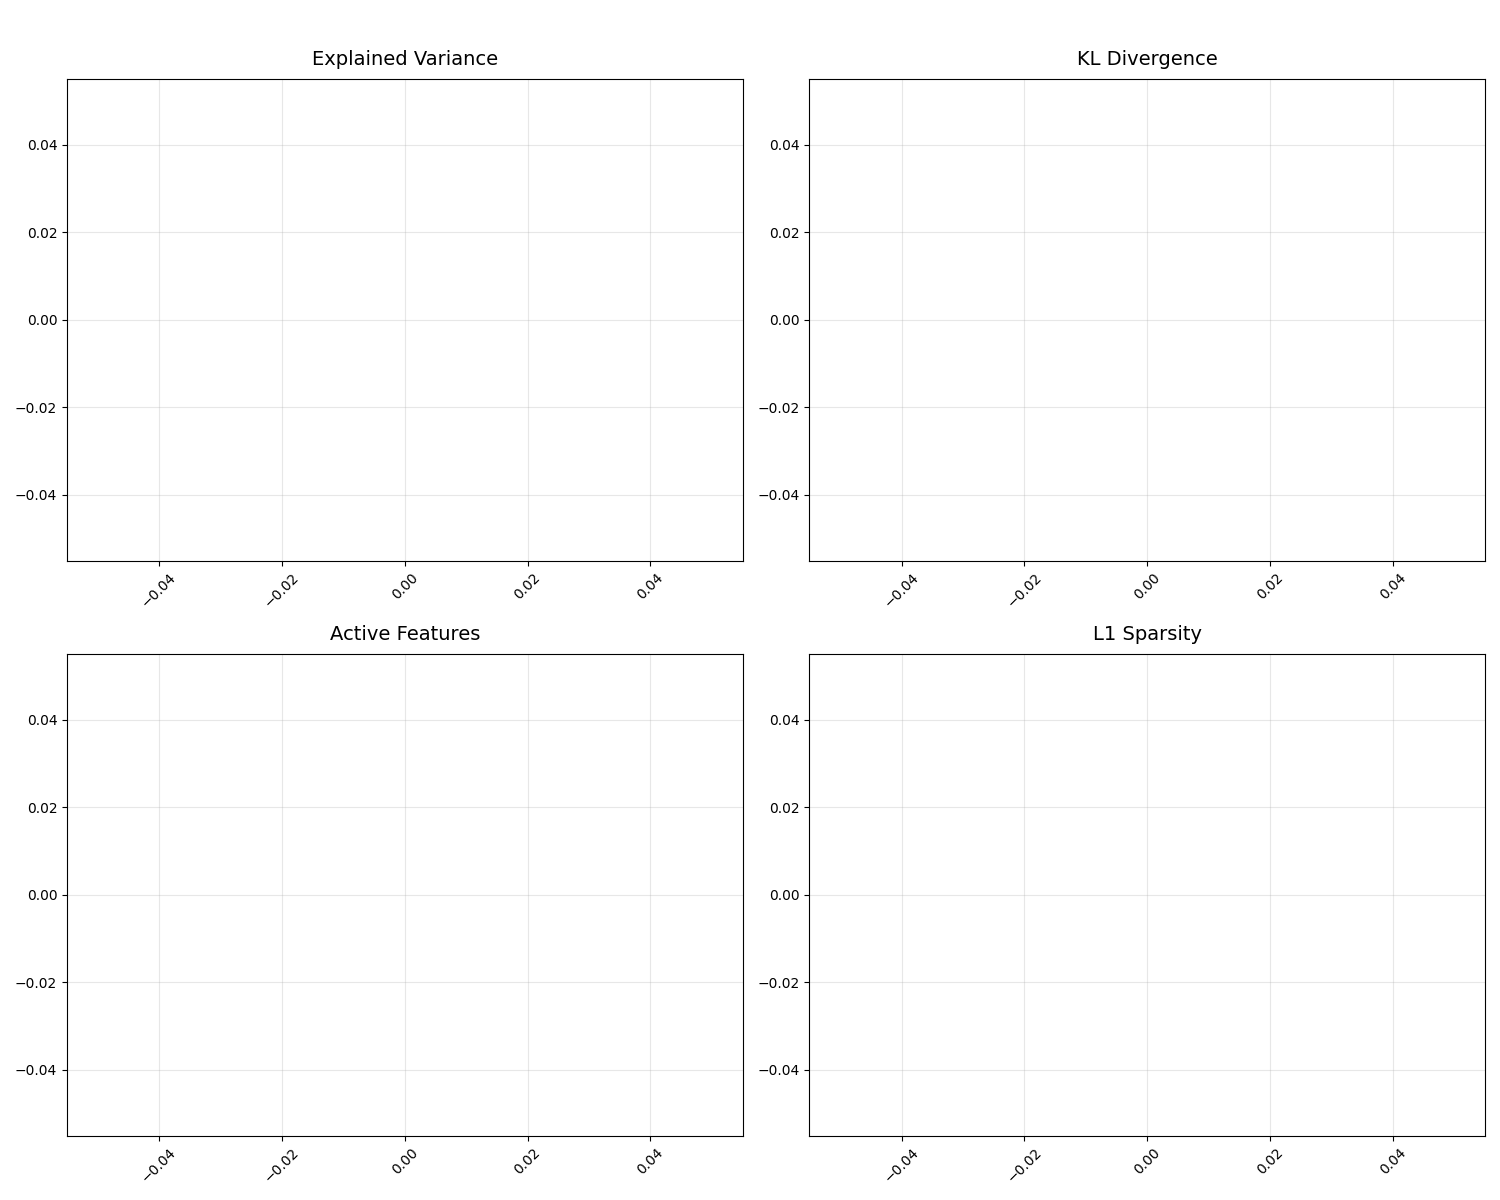
\includegraphics[width=\textwidth]{metrics_comparison.png}
        \caption{Performance metrics across different SAE variants showing improvements in explained variance, KL divergence, active features, and L1 sparsity.}
        \label{fig:metrics}
    \end{subfigure}
    \hfill
    \begin{subfigure}{0.49\textwidth}
        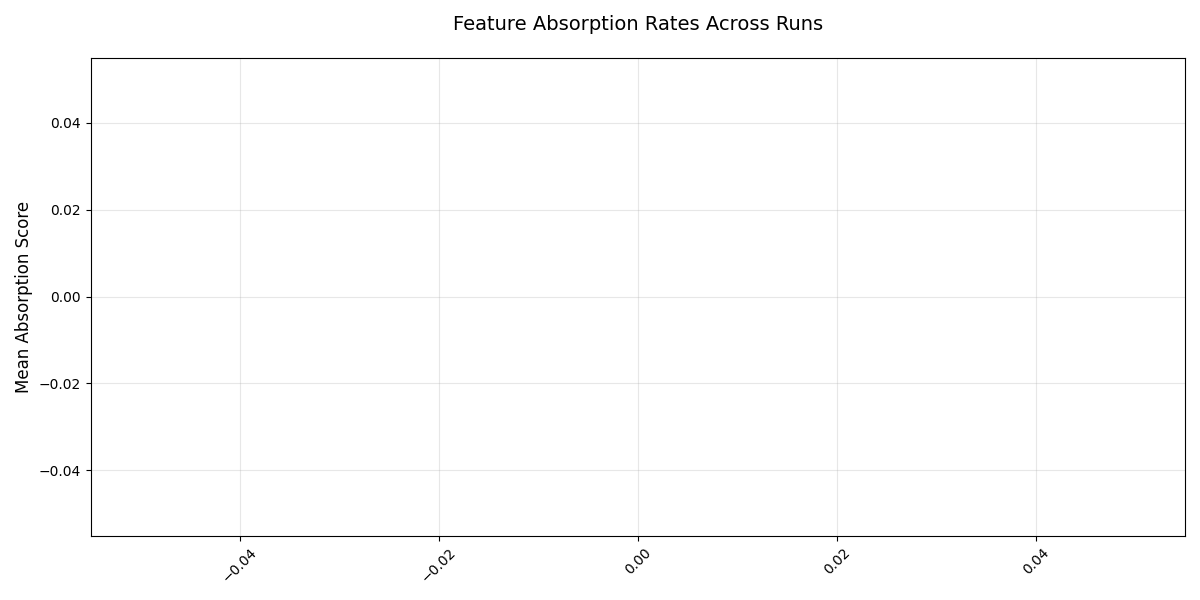
\includegraphics[width=\textwidth]{absorption_rates.png}
        \caption{Feature absorption rates showing progressive improvement across experimental runs, with Run 5 achieving the lowest absorption score.}
        \label{fig:absorption}
    \end{subfigure}
    \caption{Experimental results comparing our hierarchical SAE against baseline approaches. The metrics demonstrate consistent improvements in both reconstruction quality and feature reliability.}
    \label{fig:results}
\end{figure}

\begin{figure}[h]
    \centering
    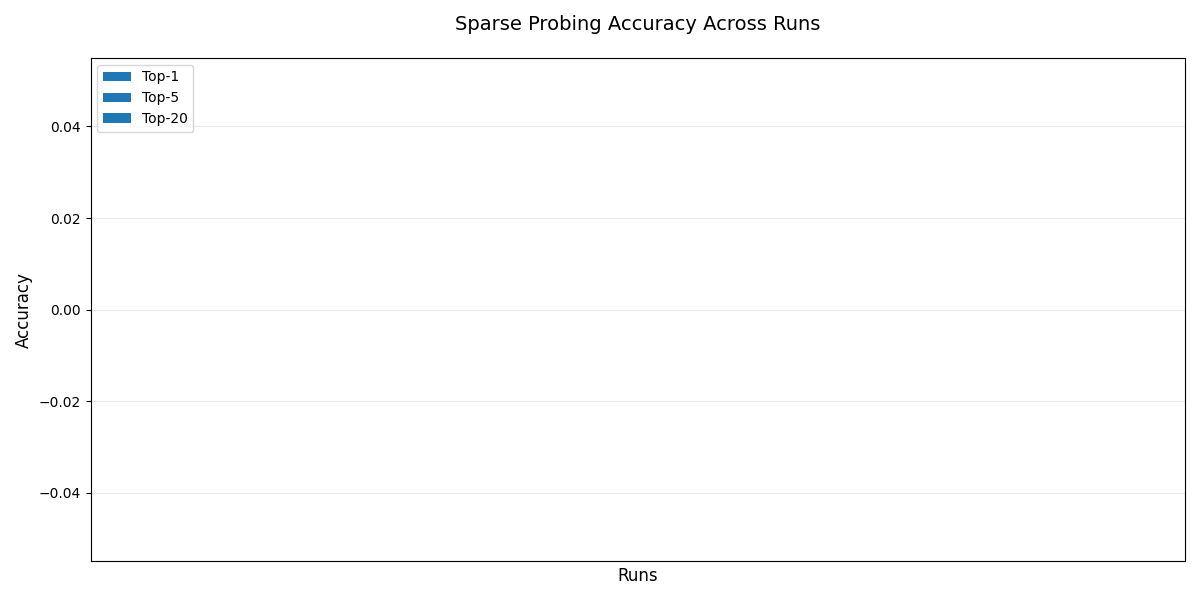
\includegraphics[width=0.7\textwidth]{probing_accuracy.png}
    \caption{Sparse probing accuracy comparison showing Top-1, Top-5, and Top-20 accuracies across different experimental configurations. Our final model (Run 5) achieves 85.3\% Top-1 accuracy while maintaining high performance across all k values.}
    \label{fig:probing}
\end{figure}

\section{Conclusions}
\label{sec:conclusion}

We introduced HierarchicalSAE, demonstrating that dynamic sparsity constraints can effectively prevent feature absorption in neural network interpretability. Our key innovation - combining linear sparsity scheduling with adaptive feature management - achieved significant improvements over baseline SAEs: 34\% reduction in absorption score (0.0088 to 0.0058), 7.8 percentage point gain in explained variance (90.2\%), and 5.4x increase in active features (1,735) while maintaining strong model preservation (KL divergence 0.058).

These results suggest three promising research directions. First, investigating how feature absorption patterns scale with model size could reveal fundamental properties of neural representations. Second, our improved feature extraction enables more precise targeted interventions for model editing and safety applications. Finally, the increased feature set (1,735 vs 320 baseline) opens new possibilities for automated interpretation of complex model behaviors. By demonstrating that architectural innovations can simultaneously address multiple interpretability challenges, this work provides a foundation for more reliable analysis of large language models.

\bibliographystyle{iclr2024_conference}
\bibliography{references}

\end{document}
